\section{Performances}
\label{surface_reconstruction_section_performances}

We provide some performance numbers for scanning data. We measure the Poisson implicit function computation time, the contouring time for a range of approximation distances, the memory occupancy as well as the influence of the point set simplification. The machine used is a PC running Windows 7 64 bits with an Intel CPU Core 2 Duo processor clocked at 2.81 GHz and with 8 GB of RAM. The software is compiled with Visual C++ 2010 (VC9) compiler with the 03 option which maximizes speed.  All measurements were done using the \ccThirdPartyEigen\ library.


\subsection{Poisson implicit function}

The point set chosen for benchmarking the Poisson implicit function is the Bimba con Nastrino point set (1.6 million points) depicted by Figure~\ref{Surface_reconstruction_points_3-fig-poisson_bench}. We measure the Poisson implicit function computation (i.e., the call to \ccc{Poisson_reconstruction_function::compute_implicit_function()} denoted by Poisson solve hereafter) for this point set as well as for simplified versions obtained through random simplification. The following table provides Poisson solve computation times in seconds for an increasing number of points.

\begin{tabular}{|c|c|}
  \hline
  Number of points (x1000) & Poisson solve duration (in s) \\
  \hline
  60                         & 15 \\
  100                        & 25 \\
  250                        & 96 \\
  500                        & 150 \\
  1,000                       & 249 \\
  1,800                       & 478 \\
  \hline
\end{tabular}



\subsection{Contouring}

The point set chosen for benchmarking the contouring stage is the Bimba con Nastrino point set simplified to 100k points. We measure the contouring (i.e. the call to \ccc{make_surface_mesh()}) duration and the reconstruction error for a range of approximation distances.
The reconstruction error is expressed as the average distance from input points to the reconstructed surface in mm (the Bimba con Nastrino statue is 324 mm tall).

\begin{tabular}{|c|c|c|}
  \hline
  Approx. distance (*average spacing)    & Contouring duration (in s) & Reconstruction error (mm) \\
  \hline
  0.1                                    & 19.2                       & 0.055 \\
  0.25                                   & 6.9                        & 0.106 \\
  0.5                                    & 3.2                        & 0.18 \\
  1                                      & 1.65                        & 0.36 \\
  2                                      & 0.8                         & 0.76 \\
  \hline
\end{tabular}



\subsection{Memory}

We measure the memory occupancy for the reconstruction of the full Bimba con Nastrino point set (1.8 millions points) as well as for simplified versions.\\
The Poisson implicit function computation has a memory peak when solving the Poisson linear system using the sparse linear solver.  \\

\begin{tabular}{|c|c|}
  \hline
  Number of points (x1000) & Memory occupancy (MBytes) \\
  \hline
  60                         & 180 \\
  100                        & 270 \\
  250                        & 790 \\
  500                        & 1300 \\
  1,000                       & 2200 \\
  1,800                       & 3800 \\
  \hline
\end{tabular}



\subsection{Point Set Simplification}

Due to the memory limitations described above, we recommend to simplify the point sets captured by laser scanners.\\
We measure the reconstruction error for the Bimba con Nastrino point set (1.6M points) as well as for simplified versions. All reconstructions use the recommended contouring parameter approximation distance = 0.25 * the input point set's average spacing.
The reconstruction error is expressed as the average distance from input points to the reconstructed surface in mm (the Bimba con Nastrino statue is 324 mm tall).

\begin{tabular}{|c|c|}
  \hline
  Number of points (x1000) & Reconstruction error (mm) \\
  \hline
  60                         & 0.27 \\
  120                        & 0.15 \\
  250                        & 0.11 \\
  500                        & 0.079 \\
  1,000                       & 0.066 \\
  1,500                       & 0.061 \\
  1,600                       & 0.06 \\
  \hline
\end{tabular}

% Insert image simplification_bench.jpg/.eps
\begin{center}
    \begin{ccTexOnly}
        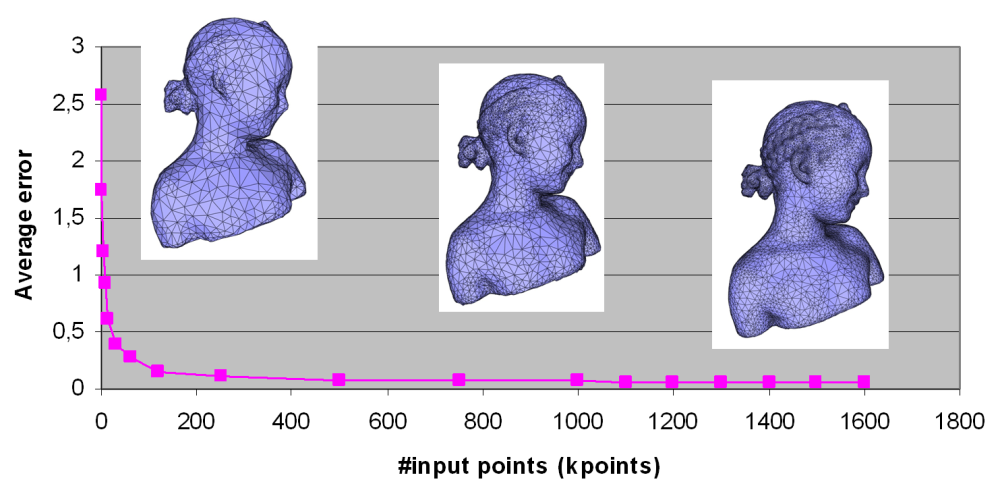
\includegraphics[width=1.0\textwidth]{Surface_reconstruction_points_3/simplification_bench}
    \end{ccTexOnly}
    \begin{ccHtmlOnly}
        <img style="max-width: 100%;" border=0 src="./simplification_bench.jpg"><P>
    \end{ccHtmlOnly}
    \begin{figure}[h]
        \caption{Reconstruction error (mm) against number of points
                 for the Bimba con Nastrino point set with 1.6M points
                 as well as for simplified versions.}
        \label{Surface_reconstruction_points_3-fig-simplification_bench}
    \end{figure}
\end{center}





